\subsection{2. Stufe - Semantische Evaluation}\label{sem_eval}
Sofern alle Typ-Konvertierungsvarianten des erwarteten Interfaces bzgl. einer Menge von angebotenen Interfaces in der 1. Stufe ermittelt wurden, k�nnen die ben�tigten Komponenten erzeugt und getestet werden.\\\\
Diese Pr�fung wird �ber die vorab spezifizierten Testf�lle des erwarteten Interfaces vorgenommen. In einem vorherigen Abschnitt wurde schon kurz beschrieben, wie eine solche Testklasse aufgebaut ist. In diesem Abschnitt wird beschrieben, wie die zu testenden ben�tigten Komponenten ermittelt werden und wie die Tests durchgef�hrt werden. 
Dies erfolgt in 6 Schritten, die im Folgenden erl�utert werden. Eine schmatische Darstellung der Semantischen Evaluation ist \abbref{flowchart_sem_eval} zu entnehmen.
\myBigFigure{flowchart_sem_eval}{Schema der semantischen Evaluation}{flowchart_sem_eval}

\subsubsection{Ermittlung der Testklassen zum erwarteten Interface}\label{sem_eval_step1}
Die Ermittlung der Testklassen erfolgt �ber die Annotation @QueryTypeTestReference, welche im erwarteten Interface spezifiziert wird. Von diesen Testklassen wird ein Testobjekt �ber den Default-Konstruktor erzeugt.
\subsubsection{Schritt 2: Kombination von Typ-Konvertierungsvarianten}\label{sem_eval_step2}
In diesem Schritt werden die ermittelten Typ-Konvertierungsvarianten miteinander kombiniert, was einer Kombination der angebotenen Interfaces gleicht. Die Anzahl $k$ der zu kombinierenden Typ-Konvertierungsvarianten kann jedoch variieren. Wenn $|EM|$ die Anzahl der Methoden im erwarteten Interface ist, gilt f�r $k$:
\begin{align*}
1 \leq k \leq |EM|
\end{align*}
\noindent
Da $k$ variabel ist, wird dieser Schritt zusammen mit allen folgenden Schritten mitunter mehrfach durchlaufen. Die Nummer des jeweiligen Iterationsschrittes wird mit $k$ gleichgesetzt. Somit wird die Anzahl der zu kombinierenden Typ-Konvertierungsvarianten mit jedem Durchlauf erh�ht. \abbref{tkv_alv_alu_1} zeigt die Kombinationen von Typ-Konvertierungsvarianten, die sich - bezogen auf die Beispiele aus \abbref{konvar_voll} und \abbref{konvar_unv} - im ersten Durchlauf ergeben. Im zweiten Durchlauf w�rde sich nur eine Kombination von Typ-Konvertierungsvarianten ergeben, da die beiden Typ-Konvertierungsvarianten von AIv und AIu miteinander kombiniert werden (siehe \abbref{comb_tkv_alv_alu_1}).



\begin{figure}[H]
\begin{minipage}[b]{.48\linewidth}
  \centering
  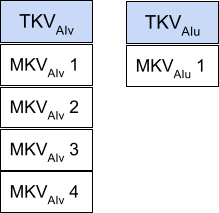
\includegraphics[width=.6\linewidth]{tkv_alv_alu_1}
  \caption{Kombinationen von Typ-Konvertierungsvarianten von AIu und AIv im ersten Durchlauf}
  \label{abb:tkv_alv_alu_1}

\end{minipage}%
\hspace{.04\linewidth}% Abstand zwischen Bilder
\begin{minipage}[b]{.48\linewidth}


  \centering
  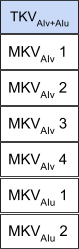
\includegraphics[width=.2\linewidth]{comb_tkv_alv_alu_1}
  \caption{Kombinationen von Typ-Konvertierungsvarianten von AIu und AIv im zweiten Durchlauf}
  \label{abb:comb_tkv_alv_alu_1}

\end{minipage}
\end{figure}

\noindent
So berechnet sich die Anzahl an ermittelten Kombinationen von Typ-Konvertierungsvarianten  ($|KombTKV|$) f�r jeden Durchlauf $k$ in Abh�ngigkeit von der Anzahl der in der 1. Stufe ermittelten Typ-Konvertierungsvarianten ($|TKV|$) wie folgt:
\begin{align*}
|KombTKV| = \frac{|TKV|! }{ (|TKV| - k)! * k!}
\end{align*}


\subsubsection{Schritt 3: Erzeugen einer ben�tigten Komponente}\label{sem_eval_step3}
Eine ben�tigte Komponente besteht aus einer Kombination von Methoden-Konvertierungsvarianten, wobei f�r jede erwartete Methode genau eine Methoden-Konvertierungsvariante innerhalb der ben�tigten Komponente existiert.\\\\
F�r die Ermittlung der Kombinationen von Methoden-Konvertierungsvarianten wird eine Kombination von Typ-Konvertierungsvarianten aus der Ergebnismenge des zweiten Schrittes im aktuellen Durchlauf  selektiert. Die daraus erzeugten Methoden-Konvertierungsvarianten werden hinsichtlich der Methoden aus dem erwarteten Interface miteinander kombiniert.\\\\
F�r die erste Kombination von Typ-Konvertierungsvarianten, die \abbref{tkv_alv_alu_1} zu entnehmen ist ($TKV_{AIv}$),  k�nnen folgende Kombinationen von Methoden-Konvertierungsvarianten erzeugt werden (siehe \abbref{comb_mkv_alv_1}).
\myBigFigure{comb_mkv_alv_1}{Kombinationen von Methoden-Konvertierungsvarianten AIv}{comb_mkv_alv_1}
\noindent
Analog dazu wird f�r die zweite Kombination von Typ-Konvertierungsvarianten, die \abbref{tkv_alv_alu_1} zu entnehmen ist ($TKV_{AIu}$), folgende Kombination von Methoden-Konvertierungsvarianten erzeugt (siehe \abbref{comb_mkv_alu_1}).\\\\
Ausgehend von der Kombination von Typ-Konvertierungsvarianten aus \abbref{comb_tkv_alv_alu_1} ($TKV_{AIu+AIv}$), sind in \abbref{comb_mkv_alu_alv} die daraus resultieren Methoden-Konvertierungsvarianten dargestellt.Zu beachten ist, dass die ersten vier Kombinationen bereits im vorherigen Durchlauf erzeugt wurden (siehe \abbref{comb_mkv_alv_1}) und dementsprechend auch getestet wurden.



\begin{figure}[H]
\begin{minipage}[b]{.38\linewidth}
  \centering
  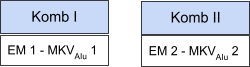
\includegraphics[width=.6\linewidth]{comb_mkv_alu_1}
  \captionof{figure}{Kombinationen von Methoden-Konvertierungsvarianten AIu}
  \label{abb:comb_mkv_alu_1}

\end{minipage}%
\hspace{.04\linewidth}% Abstand zwischen Bilder
\begin{minipage}[b]{.58\linewidth}


  \centering
  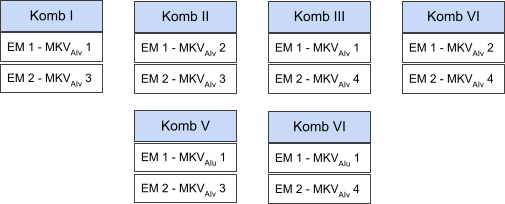
\includegraphics[width=\linewidth]{comb_mkv_alu_alv}
  \captionof{figure}{Kombinationen von Methoden-Konvertierungsvarianten AIu+AIv}
  \label{abb:comb_mkv_alu_alv}

\end{minipage}
\end{figure}


\noindent


\noindent
Im Allgemeinen l�sst sich sagen, dass die Anzahl der Kombinationen von Methoden-Konvertierungsvarianten von der Anzahl der Methoden im erwarteten Interface ($|EM|$) und der Anzahl von Methoden-Konvertierungsvarianten ($|MKV|$), die aus der selektierten Kombination von Typ-Konvertierungsvarianten erzeugt werden k�nnen. Da aus einer Kombination von Methoden-Konvertierungsvarianten jeweils eine ben�tigte Komponente erzeugt werden kann, gilt f�r die Anzahl der ben�tigten Komponenten ($|Komb_{ben}|$) dasselbe. Im schlimmsten Fall berechnet sich die Anzahl der ben�tigten Komponenten wie folgt:
\begin{align*}
|Komb_{ben}| = |Komb_{MKV}| = \frac{|MKV|!}{(|MVK| - |EM|)!*|EM|!}
\end{align*}


\subsubsection{Injizieren der ben�tigten Komponente}\label{sem_eval_step4}
Der Setter f�r die Setter-Injection wird in der Testklasse �ber die Annotation @QueryTypeInstanceSetter ermittelt. Danach wird diese Methode auf dem Testobjekt mit der ben�tigten Komponente als Parameter aufgerufen. 
\subsection{Schritt 5: Durchf�hren der Tests}\label{sem_eval_step5}
Die Testf�lle aus der Testklasse werden �ber die Annotation @QueryTypeTest ermittelt und sequentiell ausgef�hrt. Als Ergebnis der Testausf�hrung f�r eine ben�tigte Komponente wird ein Objekt des Typs TestResult zur�ckgegeben. Tritt bei der Testausf�hrung eine Exception auf, wird diese im TestResult-Objekt hinterlegt. Im Anschluss wird das TestResult-Objekt direkt zur�ckgegeben, um die Ausf�hrung der �brigen Tests zu verhindern. Wenn ein Test mit positivem Ergebnis durchgef�hrt wird, wird das Attribut passedTests im TestResult-Objekt inkrementiert. Sollten alle Tests erfolgreich durchgef�hrt worden sein, wird das TestResult-Objekt zur�ckgegeben.
\myparagraph{Umgang mit kombinierten angebotenen Komponenten}
Ab dem zweiten Durchlauf werden werden die ben�tigten Komponenten in Schritt 3 aus Kombinationen von Typ-Konvertierungsvarianten mehrere angebotener Interfaces erzeugt. Das f�hrt dazu, dass die Methodenaufrufe auf dem erwarteten Interface an unterschiedliche angebotene Komponenten delegiert werden. Hierbei kann der Fall eintreten, dass mehrere dieser Methoden von der Semantik her auf den gleichen Daten operieren m�ssen, die Aufrufe dieser jedoch an unterschiedliche Komponenten delegiert werden, welche auch auf unterschiedlichen Daten operieren.\\\\
Ein Beispiel hierf�r w�re ein Stack, der durch das erwartete Interface Stack beschrieben. Dieses enth�lt eine push und eine pop Methoden mit der ein Element im Stack hinzugef�gt bzw. entfernt werden kann (siehe \abbref{expected_stack}). Hierbei ist anzunehmen, dass die beiden Methoden auf denselben Daten arbeiten, sodass nach dem Hinzuf�gen eines Elements a (push(a)) und dem darauf folgenden Aufruf der Methode pop() als R�ckgabewert wieder das zuvor hinzugef�gte Element a geliefert wird (siehe \abbref{sd_stack_1}). Wenn die beiden Methoden-Aufrufe jedoch an zwei unterschiedliche Objekte StackA und StackB delegiert werden, die auf unterschiedlichen Daten operieren, dann w�rde dieses Verhalten nicht nachgewiesen werden k�nnen (siehe \abbref{sd_stack_2}).

\begin{figure}[H]
\begin{minipage}[b]{.24\linewidth}
  \centering
  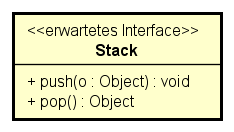
\includegraphics[width=\linewidth]{expected_stack}
  \captionof{figure}{Erwartetes Interface Stack}
  \label{abb:expected_stack}

\end{minipage}%
\hspace{.04\linewidth}% Abstand zwischen Bilder
\begin{minipage}[b]{.72\linewidth}


  \centering
  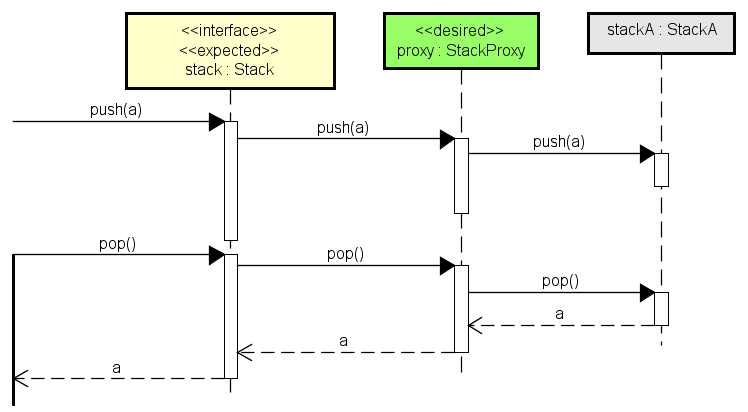
\includegraphics[width=\linewidth]{sd_stack_1}
  \captionof{figure}{Delegation der Stack-Methoden an genau eine angebotene Komponente}
  \label{abb:sd_stack_1}

\end{minipage}
\end{figure}


%\myBigFigure{expected_stack}{Erwartetes Interface Stack}{expected_stack}
%\myBigFigure{sd_stack_1}{Delegation der Stack-Methoden an genau eine angebotene Komponente}{sd_stack_1}
\myBigFigure{sd_stack_2}{Delegation der Stack-Methoden an unterschiedliche angebotene Komponenten}{sd_stack_2}
\noindent
In einem solchen Fall sollte der Zusammenhang dieser erwarteten Methoden in den Tests spezifiziert werden, sodass diese besonderen semantischen Anforderungen in diesem Schritt evaluiert werden k�nnen. \lstref{LST_StackTest} zeigt ein Beispiel bezogen auf das Szenario aus \abbref{sd_stack_1}.
\begin{lstlisting}[{caption = Testklasse f�r ein erwartetes Interfaces Stack
},{label = LST_StackTest}]
public class StackTest {

  private Stack stack;

  @QueryTypeInstanceSetter
  public void setProvider( Stack stack ) {
    this.stack = stack;
  }

  @QueryTypeTest
  public void pushPop() {
    Object a = new Object();
    stack.push( a );
    Object evalObj = stack.pop();
    assertTrue( a == evalObj );
  }

}
\end{lstlisting}

\subsubsection{Schritt 6: Auswertung des Testergebnisses}\label{sem_eval_step6}
Sofern alle Tests erfolgreich durchgelaufen sind, wird die aktuell selektierte ben�tigte Komponente als passend bewertet und als Ergebnis des Explorationsalgorithmus zur�ckgegeben.\\\\
Sollte einer der Tests nicht erfolgreich sein, wird die semantische Evaluation ab Schritt 3 (siehe \ref{sem_eval_step3}) wiederholt. Sofern keine ben�tigten Komponenten mehr erzeugt werden k�nnen, ist die Suche nach einer passenden Komponente gescheitert.\\\\
Da die Suche zur Laufzeit ausgef�hrt wird, reicht es, wenn eine passende Komponente gefunden wird. Selbst wenn es mehrere passende Komponenten geben sollte, g�be es in dem beschriebenen Verfahren keine M�glichkeit festzustellen, welche die semantischen Anforderungen besser erf�llt. Zwar w�ren k�nnte man die passenden Komponenten hinsichtlich der ben�tigten Systemressourcen untersuchen. Aufgrund der Vielzahl von m�glichen Kombinationen (siehe \ref{sem_eval_step2} und \ref{sem_eval_step3}) rechtfertigt der daf�r notwendige Aufwand den daraus resultierenden Performancegewinn vermutlich nicht.
